%Latex Template (Master file)
% By Sanjay S. Shitole : modified on 17 March 2015.
% Pl. note : this template is used for practice and to show the different functions of LaTeX. Refered citations are not actuals.
%-------------------------------------------------------------
%--------------------------------------------------------------
%Pl. refer the  database.bib file in the folder for references list
% study the syntax for refernces as shown in database.bib

%--------------------------------------------------------
%--------------------------------------------------------
% To create list of table  --
% Run the code twice (pdflatex or latex)
%%%%%%%%%%%%%%%%%%%%%%%%%%%%%%%%%%%% If you are using "TecnicCenter" editor then
%To get the references using bibtex follow following sequence.
%pdflatex
%bibtex
%pdflatex
%pdflatex
%%%%%%%%%%%%%%%%%%%%%%%%%%%%%%%%%%%%%%%%%%%%%%%%%%%%%
% Texstudio is the best editor at present
%%%%%%%%%%%%%%%%%%%%%%%%%%%%%%%%%%%%%%%%%%%%%%%%%%%
\documentclass[12pt,a4paper,final,oneside]{report}

\usepackage{geometry}
\usepackage{amsfonts}
\usepackage{amssymb}
\usepackage{graphics}
\usepackage{amsmath}
\usepackage{array}
\usepackage[pdftex]{hyperref}
\usepackage{epstopdf}
\usepackage{setspace}
\usepackage{natbib}


\begin{document}

\thispagestyle{empty}
%%%% This is first page
%%%%% Refer q31.tex file

\begin{center}
A Seminar /Project Report On

\LARGE{Topic Name}

\end{center}

\vspace{3cm}

\begin{center}

Submitted in partial fulfilment for the
\linebreak degree of Bachelor of Technology in
\linebreak  Information Technology
\end{center}
\vspace{2cm}
\begin{center}

Submitted by
\linebreak \textbf{Name of Student}
\vspace{2cm}

 Under the guidance of
\linebreak \textbf{Guide Name}
\end{center} 

\vspace{2cm}
\begin{center}

\vspace{1cm}
 


 \textbf{Name of College}
\linebreak Address 
\linebreak Address
\linebreak Year
\end{center}


%\end{document}

%%%%%%%%%%%%%% this is for certificate, pl modify according to your need
% refer q31.tex

\newpage
\thispagestyle{empty}
\begin{center}
\LARGE{ Approval        Sheet}
\end{center}


\vspace{2cm}

This is to certify that Name of Student has completed the -----
(Seminar/project)
 report on the topic `` topic name'' satisfactorily in partial fulfillment for the Bachelor's Degree in --------(dept) under the guidance of ----Guide Name during the year ----- as prescribed by ----name of university.

\vspace{3cm}

\begin{flushleft}
Guide \hspace{95.00mm} Head Of Department\newline



Guide name \hspace{90.00mm}    HOD name
\end{flushleft}



\vspace{2cm}
\begin{center}
Principal



Name of Principal
\end{center}

\vspace{2cm}
\begin{flushleft}
Examiner 1 \hspace{100.00mm} Examiner 2
\end{flushleft}

\newpage






 \begin{center}
 \LARGE{Declaration }
 \end{center}

I   declare    that  this  written  submission  represents  my          ideas  in  my  own  words  and  where 
others'  ideas  or  words  have  been  included,  I  have                adequately  cited  and  referenced  the  original                     
sources.       I  also  declare  that  I  have  adhered to  all               principles  of  academic  honesty  and  integrity     
and   have   not   misrepresented   or   fabricated   or    falsified   any   idea/data/fact/source   in   my 
submission.    I   understand   that  any   violation  of  the  above    will  be  cause  for  disciplinary  action   
 by  the  Institute  and  can  also  evoke   penal  action  from        the     sources  which  have  thus  not  been 
properly  cited  or  from  whom  proper  permission  has     not    been    taken  when    needed.

\vspace{1in}

\begin{flushright}
(Signature )
\end{flushright}

\vspace{0.3in}  

\begin{flushright}
(Name of the student )
\end{flushright}

\vspace{0.3in}  

\begin{flushright}
(Roll No)
\end{flushright}

\vspace{0.3in}  

\begin{flushleft}
Date
\end{flushleft}

\pagenumbering{roman}
%%%%%%%%%%%%%%%%%%% use for abstract
%%% refer q31.tex
\begin{abstract}

Abstract is the brief information regarding your project.
It may be in a single paragraph of
in multiple paragraph, but should give the information regarding your project in minimum possible words.



{\bf Keywords}: {\it TDM, FDM, ...}

\end{abstract}


  \addcontentsline{toc}{chapter}{Abstract}
%\clearpage
\tableofcontents
  
\listoftables
   \addcontentsline{toc}{chapter}{List of Tables}


\listoffigures
  \addcontentsline{toc}{chapter}{List of Figures}

%\def\abstract{
 % \chapter*{Abstract}
  %\addcontentsline{toc}{chapter}{Abstract}
  %\relax\markboth{ABSTRACT}{ABSTRACT}}
%\def\endabstract{\par\newpage}


%%% refer q31.tex 


% NOMENCLATURE
%\newpage
\chapter*{Nomenclature}
%\begin{flushleft}
%\textbf{\begin{LARGE}
%Nomenclature
%\end{LARGE}}
%\end{flushleft}
%
%\vspace{0.3in}

\begin{description}
\item{\makebox[0.75in][l]{$ dB  $}}  Decibel
\item{\makebox[0.75in][l]{$ \sigma_{s} $}} 3 dB Bandwidth of source
\item{\makebox[0.75in][l]{3G}} Third generation
\item{\makebox[0.75in][l]{4G}} Fourth Generation
\item{\makebox[0.75in][l]{TDM}} Time Division Multiplexing
\item{\makebox[0.75in][l]{WDM}} Wavelength Division Multiplexing
\end{description}

\addcontentsline{toc}{chapter}{Nomenclature}


\newpage

\pagestyle{plain}
\pagenumbering{arabic}
%\singlespacing
\onehalfspacing
%\doublespacing

%% refer q31.tex

\chapter{Introduction}
sanjay
Introduction should not be less that one page at least it should be one and half page. It should consists of the brief information of you project and what are the similar methods carried out. Introduction may be in the paragraphs with proper references of citation. Introduction also consists of figures which are properly captioned. 
\par It is very important to note that there should not be any space before the comma(,) or full stop (.). 
\par Last paragraph of the introduction should give flow of information in succeeding chapter.  

\section{Objectives of the Study}

\section{Organization of the report}

%% refer q31.tex

\chapter{Review of Literature Survey}
This chapter should consists the information regarding already available solutions/methods of whatever you are proposing. \par
   Another paragraph should explain what are the problems with the solution/methods proposed by others. These methods should be properly supported by proper reference.
\chapter{Amplitude Modulation}

Study the \LaTeX\ code in chapt3.tex.
It will help you for figure insertion, math using \LaTeX\ .\, Table creation,
citations, labels.
\section{Homomorphic filter} 
 %Morphological filters
By performing simultaneous gray level range compression and contrast enhancement on illumination reflection model,one can improve the appearance of an image by designing a frequency domain procedure~\cite{man87}.
An image $f(x,y)$ can be expressed as a product of illumination and reflection components~\cite{sam09}.

 % NOTE2: pl.refer that  $ $ sign for mathamatical term in the text in line.

\begin{equation}
f(x,y)=i(x,y)r(x,y)
\end{equation}

% NOTE3:- \[ f(x,y)=i(x,y)r(x,y) \]
% this has the same effect as above code i.e
%  \begin{equation}
% f(x,y)=i(x,y)r(x,y)
% \end{equation}

here $ i(x,y) $ is  illumination component and  $ r(x,y) $ reflection component.\\

% NOTE 4: Observe the  \\  at the end
% this will help the latex to go to new line.


Fourier transform of the product of two functions is not separable, So we can define shown in as shown in Equation~\ref{fourier}

\begin{equation}
F.T[z(x,y)]=F.T[ln f(x,y)]=F.T[ln i(x,y)]+F.T[ln r(x,y)]
\label{fourier}
\end{equation}

\begin{equation}
Z(u,v)=F_{i}(u,v)+F_{r}(u,v)
\end{equation}


 \begin{equation}
  S(u,v)=H(u,v)Z(u,v)
 \end{equation}

% Note5: Observe the following code ,
% here for the equatins \[                      \] brackets are used
% this will help you if you are not interested in numbering of the equations.
% observe the effect in output pdf file.


 where $S(u,v)$ Fourier Transform of result  and $H(u,v)$ Filter function

      \[S(u,v)=H(u,v)F_{i}(u,v)+H(u,v)F_{r}(u,v)\]

      \[s(x,y)=F^{-1}[S(u,v)]\]

      \[s(x,y)=F^{-1}[H(u,v)F_{i}(u,v)]+F^{-1}[H(u,v)F^{r}(u,v)]\]

      Say
      \[i'(x,y)=F^{-1}[H(u,v)F_{i}(u,v)]\]

       \[r'(x,y)=F^{-1}[H(u,v)F_{r}(u,v)]\]

       Hence,
       \[s(x,y)=i'(x,y)+r'(x,y)\]

       Therefore,
       Let $g(x,y)$ be the inverse exponential operation

       \[g(x,y)=e^{s(x,y)}\]

      \[g(x,y)=e^{i'(x,y)}e^{r'(x,y)}\]

       \[g(x,y)=i_{0}(x,y)+r_{0}(x,y)\]

       where $i_{0}(x,y)=e^{i'(x,y)}$ and $r_{0}(x,y)=e^{r'(x,y)}$


%  Note 6:following five lines are responsible for graphics insertion.

\begin{figure}[h]
	\centering
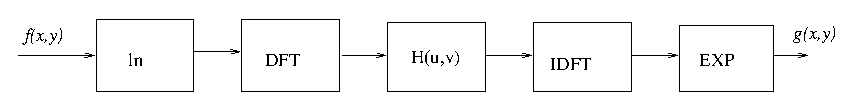
\includegraphics{blockdig.eps}
\caption{Block digram}
	\label{bbb}
\end{figure}

\begin{itemize}
\item This approach is used for homomorphic filtering as shown in figure~\ref{bbb}. The key to the approach is separation of the illumination and reflection components. Between them $i(x,y)$ contributes to the low frequency since illumination is more or less uniform and $r(x,y)$ is high frequency component as it tends to vary abruptly at junctions of dissimilar objects.
\item $H(u,v)$ is the homomorphic filtering function.A typical homomorphic filter $H(u,v)$ is as shown in figure below. Generally, $\gamma_L<1$ and$\gamma_H>1$, $H(u,v)$ tends to decrease the contribution made by low frequencies and amplify the contribution made by high frequency.
\end{itemize}

%NOTE 7: The following five lines are responsible for graphics insertion.
% Also note that in caption q312 is the figure number and after : put name of the figure.

\begin{figure}[htbp]
\centering
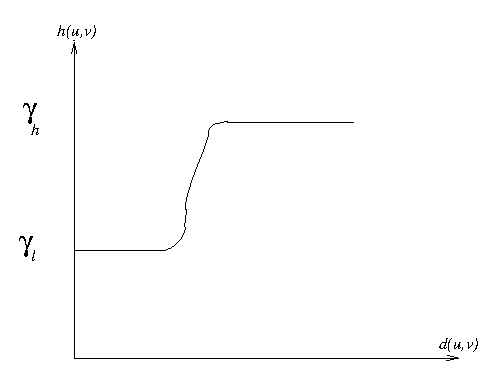
\includegraphics{graph.eps}
\caption{Transfer function}
\label{fig:graph}
\end{figure}

\section{Morphological Filters}

To understand morphological filters we first need to understand the operations dilation, erosion,opening  and  closing.

\subsection{Dilation}
With $A$ and $B$ as sets in $Z^{2}$,the dilation of $A$ and $B$ denoted as $A\oplus B$ is defined as

\[A\oplus B={Z/(\hat{B}_{z}\cap A \neq \phi}\]

Equation obtained by reflection of $B$ about origin and shifting reflection by $ z$ .
$B$  and $A$ should overlap by at least one element.Set $B$ is the structuring element in all morphological operations.\\
 \textbf{Erosion} For sets $A$ and $B$ in $Z^{2}$,the erosion of $A$ by $B$ denoted as $A\ominus B$ is defined as

\[ A\ominus B={Z/(B_{z}\subseteq A )} \]
This equation indicates that the erosion of $A$ by $B$ is the set of all points $z$ such that $B$,translated by $z$ is contained in $A$ Erosion shrinks an image.

\subsection{Opening and closing}

Opening smooths the contour of an object.
 Closing also tends to smooth sections of contours but it generally fuses narrow breaks and long thin gulfs,eliminates small holes and fills gaps in contour.
Opening is denoted by $A\circ B$

\[A\circ B=(A\ominus B)\oplus B\]

  i.e. Erosion followed by dilation
 Closing is denoted by $A\bullet B$

 \[A\bullet B=(A\oplus B)\ominus B\]

 i.e Dilation followed by erosion.
 Morphological operations can be used to construct filters.

\begin{enumerate}
	\item Suppose we have a binary image which is corrupted by noise.The noise manifests itself as light elements on a dark background and dark elements on  light components of image .
	\item A morphological filter consisting of opening followed by closing operation eliminates the noise and its effect on the image while distorting it as little as possible.
	\item The steps are as follows

\begin{itemize}
	\item We have a structuring element
	\item We erode A with the structuring element.The background noise gets eliminated in the erosion stage of opening because in this case all noise components are physically smaller then the structuring element.
For e.g. in some images the size of the noise elements actually increases.This is because these elements are inner boundaries that should increase in size as object is eroded.
\item This enlargement is countered by performing dilation.The noise components in the image are reduced in size or deleted completely.
The two operations constitute ~``opening'' A by B.
\item Net effect of opening is to eliminate all noise components in both the background and image itself.However,new gaps may be formed.
\item To counter this effect we perform dilation on the opening.Sometimes most breaks are restored but ridges are thickened.
This thickening is countered by erosion.
\item The above two steps are the closing operation.
\end{itemize}

\end{enumerate}
Hence the final result is remarkably clean of noise specs.
 Disadvantage of this filter is that some of the point ridges might not be fully repaired and can contain breaks. \\

%Note 8: If u want to insert a table your editor will help u to create %a required code for that
% for example refer the following
% go to the wizard menu and use Quick Tabular

The Table~\ref{tab:listOfStudents} is used to explain how table can be created in Latex and also observe how table in the document can be referred  in text.


\begin{table}[htbp]
	\centering
		\begin{tabular}{|c|c|c|}
			\hline Roll No & Name of the student & marks \\
			\hline 1 & Sonal & 95 \\
			\hline 2 & Komal & 97 \\
			\hline
\end{tabular}
\caption{list of students}
\label{tab:listOfStudents}
\end{table}


Refer the~\cite{sanjay} for the different \LaTeX\ templates.


The system~\cite{sanjay12} is very good.

%Note9 With a little pactice of this code you will get the idea about how to 
% use $ $, \[  \],  \\ ,
% how to insert graphics and  create Tables.
%Note10: If u are creating table of contents, List of Figures,cross reference, Citation, ...,
%then run the same code for two times.
%% refer q31.tex

\chapter{Realisation/Implementation of the proposed (name of the system) system}
   This chapter should consists of minute details of the design and development of the project supported by  diagrams  and design details. Same chapter should also consists of the testing if any necessary and results taken of any data.
%% refer q31.tex

\chapter{Conclusion and Future scope}
Should consists of two paragraph one regarding conclusion may from theory point of view or from experimentation point of view. \par
     Other paragraph should explain any task not completed due to some reasons and how it can be completed in future or some modifications in the system to improve the performance.


%% refer q31.tex
%% include the topic name as per u r project in appendix

\appendix
\chapter{Important Terms}
To compare quantitatively ..... techniques, following a set of criteria are established to ...


\chapter{Maths}
.....


\renewcommand{\bibname}{References}

%\bibliographystyle{plain}
\bibliographystyle{plainnat}
%\bibliographystyle{agsm}

\bibliography{database}
\renewcommand{\bibliography}{\References}
\addcontentsline{toc}{chapter}{References}
%% refer q31.tex

\newpage
\begin{center}
\textbf{\begin{LARGE}Acknowledgement\end{LARGE}}
\end{center}

\vspace{3cm}
I have a great pleasure to express my gratitude to all those who have contributed and motivated during my project  work. Here you have a liberty to write anything and express your feeling to all those who have helped you.



 ...\vspace{1in}\\
\\
\\
\\
\\

\begin{flushleft}
Date:
\end{flushleft}

\begin{flushright}
\begin{large} Name of Candidate\end{large}
\end{flushright}






\end{document}

